\section{EUROPA}
\label{sec:europa}

EUROPA is a general purpose AI planning toolkit developed at NASA Ames.  Automated Planning can be reformulated as a constraint satisfaction problem (TODO: ref). EUROPA is an extension of that idea, however, unlike other approaches where the entire planning problem is translated into a CSP and then solved using traditional CSP methods, EUROPA uses a constraint reasoning engine as a fundamental building block, and enriches it with other architectural components that allow a more direct mapping for scheduling and planning problems, which in turn allows easier development of efficient solving methods.

Let's look at some of the problems that can be tackled using EUROPA.

Constraint Satisfaction: 
In the N-Queens problem, chess queens must be placed on an NxN chessboard in a way that there are no queens attacking each other.

Below is an example of a random positioning of queens on a NxN chessboard. Queens in violation of the non-attack constraint are highlighted in red.

\begin{figure}
\centering
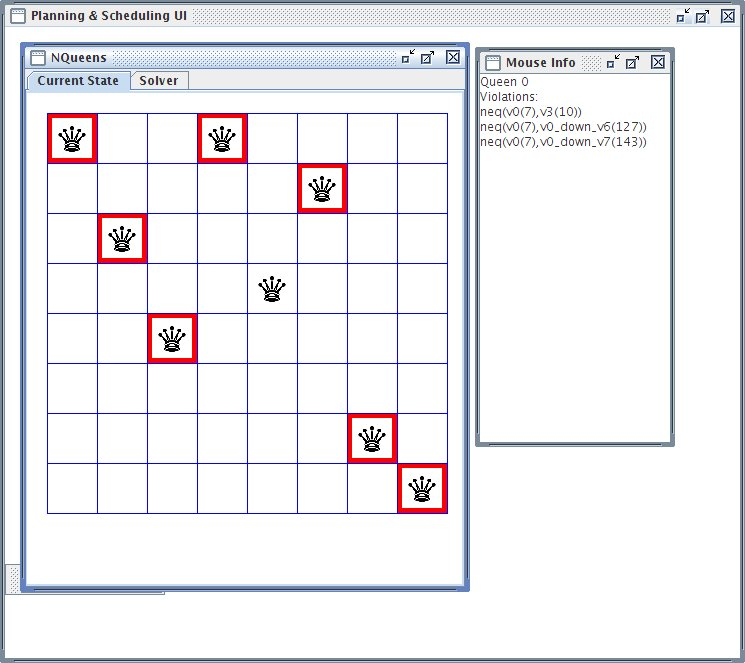
\includegraphics[scale=0.35]{figs/Example-NQueens0.jpg}
\caption{\small N-Queens problem}
\label{fig:nqueens-1}
\vskip+0.1cm
\end{figure}


If we define NxN variables Qrc, r E [1,N], c E[1,N] , 
Qrc = 1 if Cell r,c in he chessboard is occupied by a Queen, 0 otherwise.

then we have to satisfy the following constraints:
Sum(Qrc) = 1 ForAll r (Only one Queen per row)
Sum(Qrc) = 1 ForAll c (Only one Queen per column)

Sum(Qr+i,c+i) = 1
Sum(Qr-1,c+i) = 1 (only on Queen on each diagonal)

We can solve the problem by finding assignments for all variables Qrc that satisfy the constraints above. 

Below is a solution found by EUROPA using that formulation and a specialized search procedure.

\begin{figure}
\centering
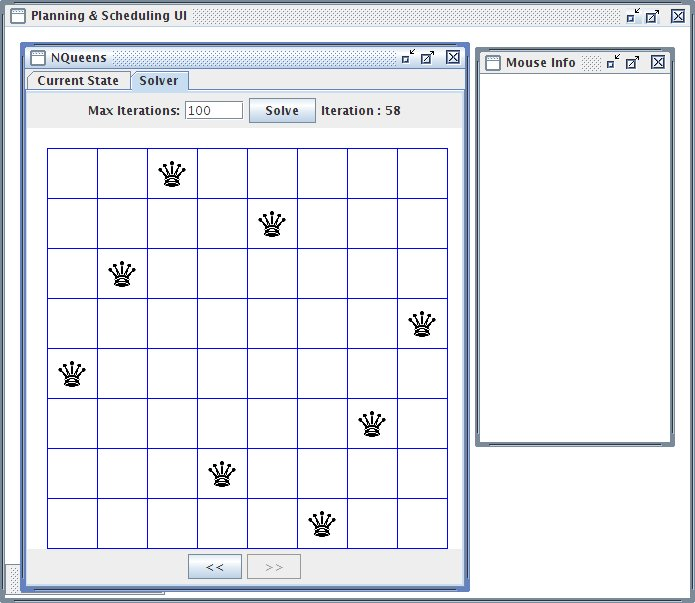
\includegraphics[scale=0.35]{figs/Example-NQueens1.jpg}
\caption{\small N-Queens solution}
\label{fig:nqueens-2}
\vskip+0.1cm
\end{figure}


Scheduling:
In the Resource Constrained Project Scheduling Problem (RCPSP), a project consisting of a set of activities must be scheduled in a way that satisfies minimum and/or maximum temporal separation constraints. The activity schedule must also respect fixed limits on the availability of resources required to perform each activity. In addition to satisfying temporal and resource constraints, it is common for the user to want to minimize makespan so that the entire project is finished as early as possible.

Below is an example of a a solution provided by EUROPA for an RCPSP instance with 10 activities, 5 resources and 30 temporal constraints.

\begin{figure}
\centering
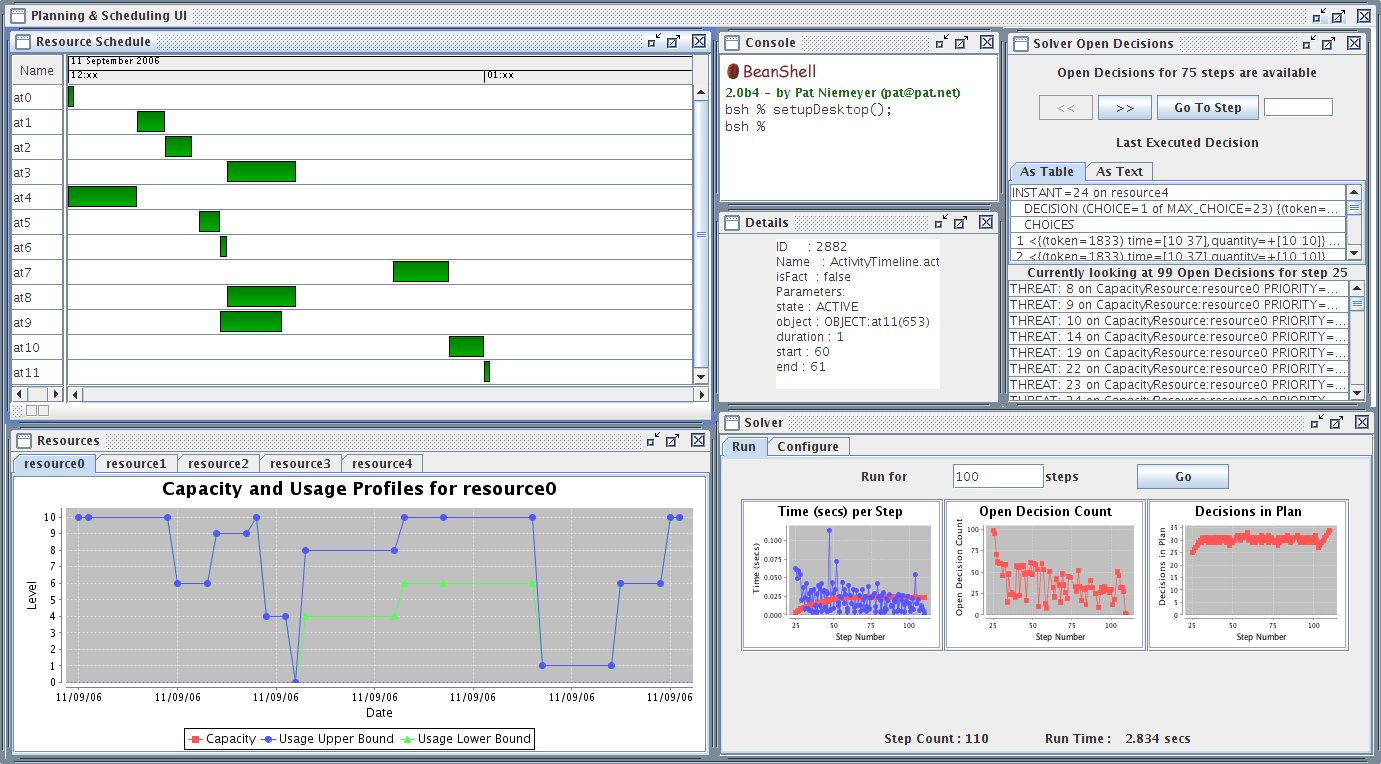
\includegraphics[scale=0.35]{figs/Example-UBO0.jpg}
\caption{\small RCPSP problem}
\label{fig:rcpsp-1}
\vskip+0.1cm
\end{figure}


Planning:
In the Shopping Agent Problem (TODO: ref to Norvig) an agent needs to purchase a set of products that are available at specific locations (supermarket, hardware store, etc), the agent  is subject to temporal (must complete tasks by specific deadlines) and resource (fuel, carrying capacity, etc) constraints. The agent must figure out what actions need to be performed to find and acquire the required items, as well as when to perform each of those actions.

Below is a solution produced by EUROPA for a simple problem instance where the shopping agent needs to buy Bananas, Milk and a Drill.

\begin{figure}
\centering
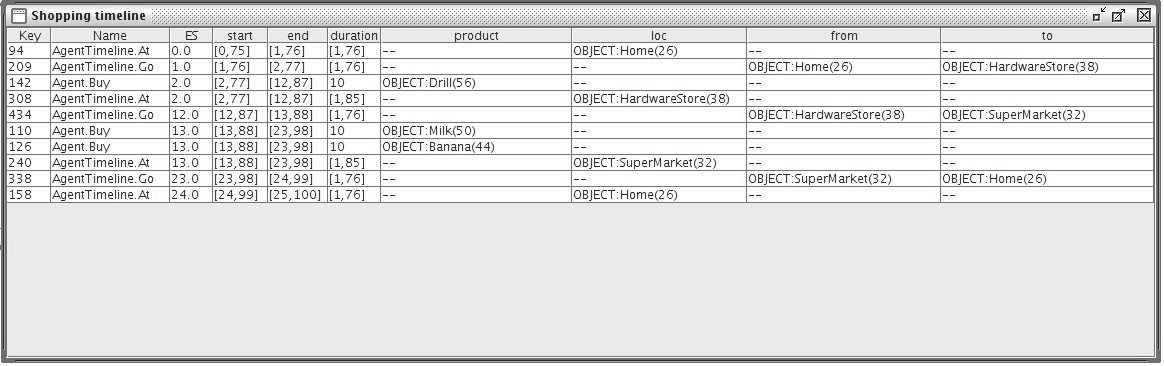
\includegraphics[scale=0.35]{figs/Example-Shopping0.jpg}
\caption{\small Shopping Agent problem}
\label{fig:shopping-1}
\vskip+0.1cm
\end{figure}


As we can see, a planning problem (what actions must be performed to achieve a goal) may embed a scheduling problem (in what order should those actions be performed), and both planning and scheduling embed Constraint Satisfaction problems since temporal, resource and many other kinds of constraints must be respected in most real life problems.

These relationships between Planning, Scheduling and Constraint Satisfaction have been examined in detail in the literature (TODOL ref Frank et al on Planning vs. Scheduling), and they lead to EUROPA's use of constraint reasoning as its innermost building block. Next we will examine the main ideas from Constraint Satisfaction Programming, and from Constraint Based Planning and Scheduling that constitute EUROPA's theoretical underpinnings, then we dive into how EUROPA implements those ideas.

\subsection{Constraint Programming}
\label{sec:europa:cp}

Constraint Satisfaction Programming, also know as Constraint Programming (CP) is a discipline that provides a generic framework for representing, solving and making logical inference on constraints. A complete treatment of this discipline is given in [MAR98] and [APT03] and very concise introductions are provided in [BAR99] and [LUS01]. 

	A constraint programming problem consists of a set of variables V={x1,..,xN}, where each variable takes values from a domain d1,..,dN. Domains are most often discrete and finite, but there are numerous CP implementations associated with continuous domains. Given a defined conjunctive set of constraints on the variables: $C=\{c1(x1,..,xN), ..., cK(x1,..,xN)\}$, the objective is to find one or more value assignments to V where all constraints are satisfied.

To solve a problem, CP uses logical inference to perform 2 operations:

\begin{enumerate}
	\item Bounds propagation: To infer upper and lower variable bounds. For example, from the constraints x1 + x2 <= 2, xi>=0, we can infer [0,2] bounds for x1 and x2

	\item Domain reduction: To infer a valid set of values for a variable. For example, for discrete variables, the constraints allDifferent(x1,x2,x3) and xi>=0, xi <=4. if x1 =1 and x2=3 we can infer that the valid domain for x3 is reduced to {2,4} 

\end{enumerate}

CP is normally implemented as part of a programming language and constraints are normally represented as objects [PUG95]. Any constraint can be introduced and, as long as the bounds propagation and domain reduction protocols specified by the host CP system are enforced, it will be indistinguishable from any other �primitive� CP constraint, such as <= or >=.

Solving a CSP is NP-Hard in theory, but often very efficient in practice using a number of algorithms and techniques that are well understood.

TODO: talk about arc consistency algorithms, computational complexity and solvers.


\subsection{Constraint-Based Attribute and Interval Planning}
\label{sec:europa:cp}

There has been 
State Variable representation

CSP encodings

Constraint Based and interval planning.

\subsection{EUROPA's Plan Representation}
\label{sec:europa:pr}

Variables

Values that need to be represented to describe the problem domain and over which we may want to specify constraints.

Objects

The things we wish to describe and refer to in a domain are considered Objects. As in the case with object-oriented analysis and design, one can seek out the nouns in any domain description to find likely objects. In a Mars rover example, we might consider the satellite, the camera, and the attitude controller (which orients the robot for taking pictures) to be objects. Objects have state and behavior. For example, a camera can be:

    off,
    ready, or
    taking a picture. 

An attitude controller can be:

    pointing at a position, or
    turning from one position to another. 

An object is an instance of a class. In EUROPA we model using the abstraction of a class to speak about all instances having certain properties of state and behavior. In order to describe such state and behavior we build on the formalism of first order logic.


Temporally Qualified Predicates and Actions

A predicate defines a relation between objects and properties. In EUROPA, we define such relations between variables whose domains are sets of objects and sets of properties. For example, we might use a predicate Pointing(a,p) to indicate that a rover's attitude controller a is pointing at position p. Note that a is a variable which may have a number of possible values in a problem with multiple satellites. Similarly, p is a variable whose values are the set of possible positions. In a grounded plan, single values will be specified for each variable as we saw in the case of a solved Constraint Satisfaction Problem.

In general, is is not sufficient to state that a predicate is true without giving it some temporal extent over which it holds. Predicates that are always true can be thought to hold from the beginning to the end of time. However, in practice, the temporal extent of interest must be defined with timepoints to represent its start and end. So we might want to write Pointing(a,s,e,p) to indicate that the attitude controller a is pointing at position p from time s to time e. In fact, this pattern of using such predicates to describe both state and behavior of objects is so prevalent in EUROPA that we have introduced a special construct called a Token which has the built in variables to indicate the object to which the statement principally applies and the timepoints over which it holds. In EUROPA, all predicate instances are Tokens.


Tokens

A Token is an instance of a predicate or an action and is defined over a temporal extent. Every token has five built-in variables:

    start: The beginning of the temporal extent over which the predicate is defined.
    end: The end of the temporal extent over which the predicate is defined.
    duration: The constraints start + duration = end is enforced automatically.
    object: made. The set of objects to which a token might apply. In a grounded plan each Token applies to a specific Object, reflecting the intuition that we are using Tokens to describe some aspect of an Object (i.e. its state or behavior) in time. However, in a partial plan, the commitment to a specific object may not yet have been made.
    state: Tokens can be ACTIVE, INACTIVE, MERGED, or REJECTED. The state variable captures the token's current state and its reachable states through further restriction. See the Token State Model discussion below for details. 

Objects (continued)

As we have noted, Tokens describe some aspect of an Object in time. Objects thus may have many Tokens in a plan in order to describe their state and behavior throughout all points in time of the plan. Within this general framework, we note a few particulars:

    Static Facts: Classes without predicates lead to Objects without Tokens. This arises where an objects state or behavior is independent of time. For example, a domain may have a set of locations and/or paths for which there is nothing more to say than that they exist.
    Timelines: Often objects in a domain must be described by exactly one token for every given timepoint in the plan. Such objects are so common that we provide a special construct in EUROPA to extend these semantics to derived classes. Any instances of a class derived from a Timeline will induce ordering requirements among its tokens in order to ensure no temporal overlap may occur among them. See below for further discussion.
    Resources: Metric resources, e.g. the energy of a battery or the capacity of a cargo hold, are objects with an explicit quantitative state in time and with a circumscribed range of changes that can occur to impact that state i.e. produce, consume, use, change. These changes are captured as tokens. Resources are such a common requirement for EUROPA users that special constructs are also provided for them. Instances of classes derived from a Resource will induce ordering requirements on their Tokens in order to ensure that the level of the resource remains within specified limits. 

Dynamic Objects

TODO (there was a stub in the old doxygen docs for this)
Timelines

It may be sufficient to maintain only a partial-order among tokens. However, it is often the case that tokens represent states and actions of a single object in the system. Such tokens are typically mutually-exclusive. EUROPA uses a Timeline structure developed in (??) to concisely capture system components whose behavior is described over time in this manner.

For example, consider the tire-world domain. The tire was located in the trunk with the predicate tireLocated(Trunk) and located on the ground with the predicate tireLocated(Ground). Clearly, the same tire cannot be in both places at once. A Timeline provides a simple method for aggregating the statements about a tire such that they are mutually exclusive.

Figure 1: A Timeline for a Tire

Figure 1 illustrates how a Timeline can be used to describe the whereabouts of a tire. The tire is an object in the tire-world represented as a timeline. It has predicates associated with it which can describe its states and actions over time. The predicate names need not contain the tire prefix; this is now implicit since the tokens are assigned to a specific tire instance (i.e. an instance of a Timeline). While Timelines are a useful element of the EUROPA planning paradigm, they are not essential. A more general notion of a system Object can be used which does not impose restrictions of mutual-exclusion or non-zero duration. This can be important in supporting partial-order planning.

For this example, the state of the tire is specified using 3 contiguous tokens. The end and start time-points are related by an equality constraint. A Moving predicate has been introduced to cover the transition from one location to another. It takes 2 location arguments. Notice that precedence relationships exist between tokens such that they cannot overlap but the start and end times may remain flexible. To illustrate this, sample times are included. Assume a total time range of interest between 0 and 1000. In addition, tokens on Timelines have a minimum duration of 1. As a result the values shown are the most flexible possible values for the start and end of each token. There are a number of advantages of allowing this flexibility. First, the basic structure of the plan can be developed without over-committing to specific times. If it is not necessary for the tire to be on the ground at time-step 4, then a planner should not be forced to specify it. Such an approach permits a least-commitment approach to planning. Second, in many domains it is simply impossible to know in planning exactly how long an activity might take. For example, a common activity of driving a car from one point to another on a road can take varying amounts of time depending on traffic and traffic lights. In such circumstances it is more practical to express upper and lower bounds on durations which naturally lead to intervals for start and end times. In such domains, flexibility in planning aids robustness in execution.
Rules

In order for a plan to be valid, it must comply with all rules and regulations pertinent to the application domain in question. Rules govern the internal and external relationships of a token. For example, consider a parameterized predicate describing a transition from one location to another. Let the parameters be from and to. The parameters are instantiated on a token as variables whose domain of values is the set of all locations in a given problem. A rule governing an internal relationship among token variables might stipulate that a transition must involve a change in location. This can be easily expressed as a constraint on the definition of a predicate of the form: from != to. It is reasonable to further stipulate that one must be Located somewhere before a transition can occur, and one must end up Located somewhere when completed. This is an example of a rule governing an external relationship among tokens. It specifies a requirement that tokens of the predicate Located precede and succeed tokens of the predicate Moving.

Figure 2: Internal and external relationships from rules on Moving Figure 2 illustrates the entities and relations involved in specifying such a rule on a Moving predicate. The token on which the rule applies is referred to as the master. Each Located token required by the master is referred to as a slave. All variables are indicated by name and their domains are expressed as intervals in the case of temporal variables and as enumerations for the remainder. Application of a rule on a token can thus cause slave tokens, variables, and constraints to be introduced.
Token State Model

The capability of a domain rule to cause a slave token to be created is a key vehicle through which planning occurs. Semantically, this rule imposes a requirement for supporting tokens to be in the plan in order for the master to be valid. There are 2 possibilities to consider:

    The slave is inserted as an active token in the plan. As such, rules may be activated on the slave, and it may consume resources.
    The token is merged with a matching token already in the plan. Once a slave is merged, the requirement it represents are considered satisfied. The process of merging passes on all restrictions imposed on the slave to the active token upon which it is merged. Merging a token requires finding a target active token that is compatible with the inactive token. For an active token and an inactive token to be compatible requires that they are instances of the same predicate and that no intersections between corresponding variables are empty. The effect of merging is illustrated in Figure 3. 

Figure 3: Merging an inactive token on an active token. Domain restrictions occur in highlighted variables of active token.

On creation of a token, where the commitment has not been made yet to activate or merge the token, the token is said to be inactive. There is a nuance to the state model for tokens which relate to the mode of its creation. If the token is allocated explicitly by an external actor, rather than internally through rule firing, it may include the state rejected indicating the planner is permitted to reject the token. A valid plan can include rejected tokens. This typically arises where the token represents a goal that is preferable to achieve but not mandatory. This state is not reachable for slaves since that would imply selective adherence to the domain model. Figure 4 presents the state transition diagram for token states relevant for planning. The transitions are operations on a partial plan which can decide an outcome for an inactive token. As operations which may arise in search, they must be reversible during backtracking. The cancellation operations in each case are also shown.

Figure 4: Token States and Transitions for Planning

The state of a token is embodied with a 5th and final built-in variable referred to as the state variable. The planner states are values in the domain of this variable {MERGED, ACTIVE, REJECTED}. The INACTIVE state is captured by the variable being unbound. If a value is removed from the domain, that state will not be reachable. For example, when a slave is created via a rule, the REJECTED value is removed from its state variable.
Summary

This page has presented the main elements of the EUROPA planning approach. They are:

    Temporally scoped predicates and actions (a.k.a. Tokens) to represent states and actions in time. Note that tokens do not discriminate between state and action.
    Constraints to describe relationships among tokens. This provides an expressive method of describing interactions among tokens in the context of Temporal Planning.
    Timelines as a concise abstraction to express the evolution of state and behavior for a system component. It provides semantics of mutual exclusion sequencing in time. Other core abstractions are available in EUROPA for handling metric resources.
    Domain rules to describe internal and external relationships on and between tokens respectively. Rules are applied to active tokens (master tokens) referred to as masters and typically produce inactive tokens (slaves) which are a key vehicle through which the planning process evolves. The rule structure in EUROPA differs from the more restrictive commitment to preconditions and effects in classical planning which prohibits durative actions and disembodied effects (i.e. effects which may not occur until some temporal distance after the end of the action).
    Token States which are the basis of planning operations on a partial plan. 

\subsection{EUROPA's Architecture}
\label{sec:europa:arch}

The following figure displays the main architectural components in EUROPA and their relationships:


\begin{figure}
\centering
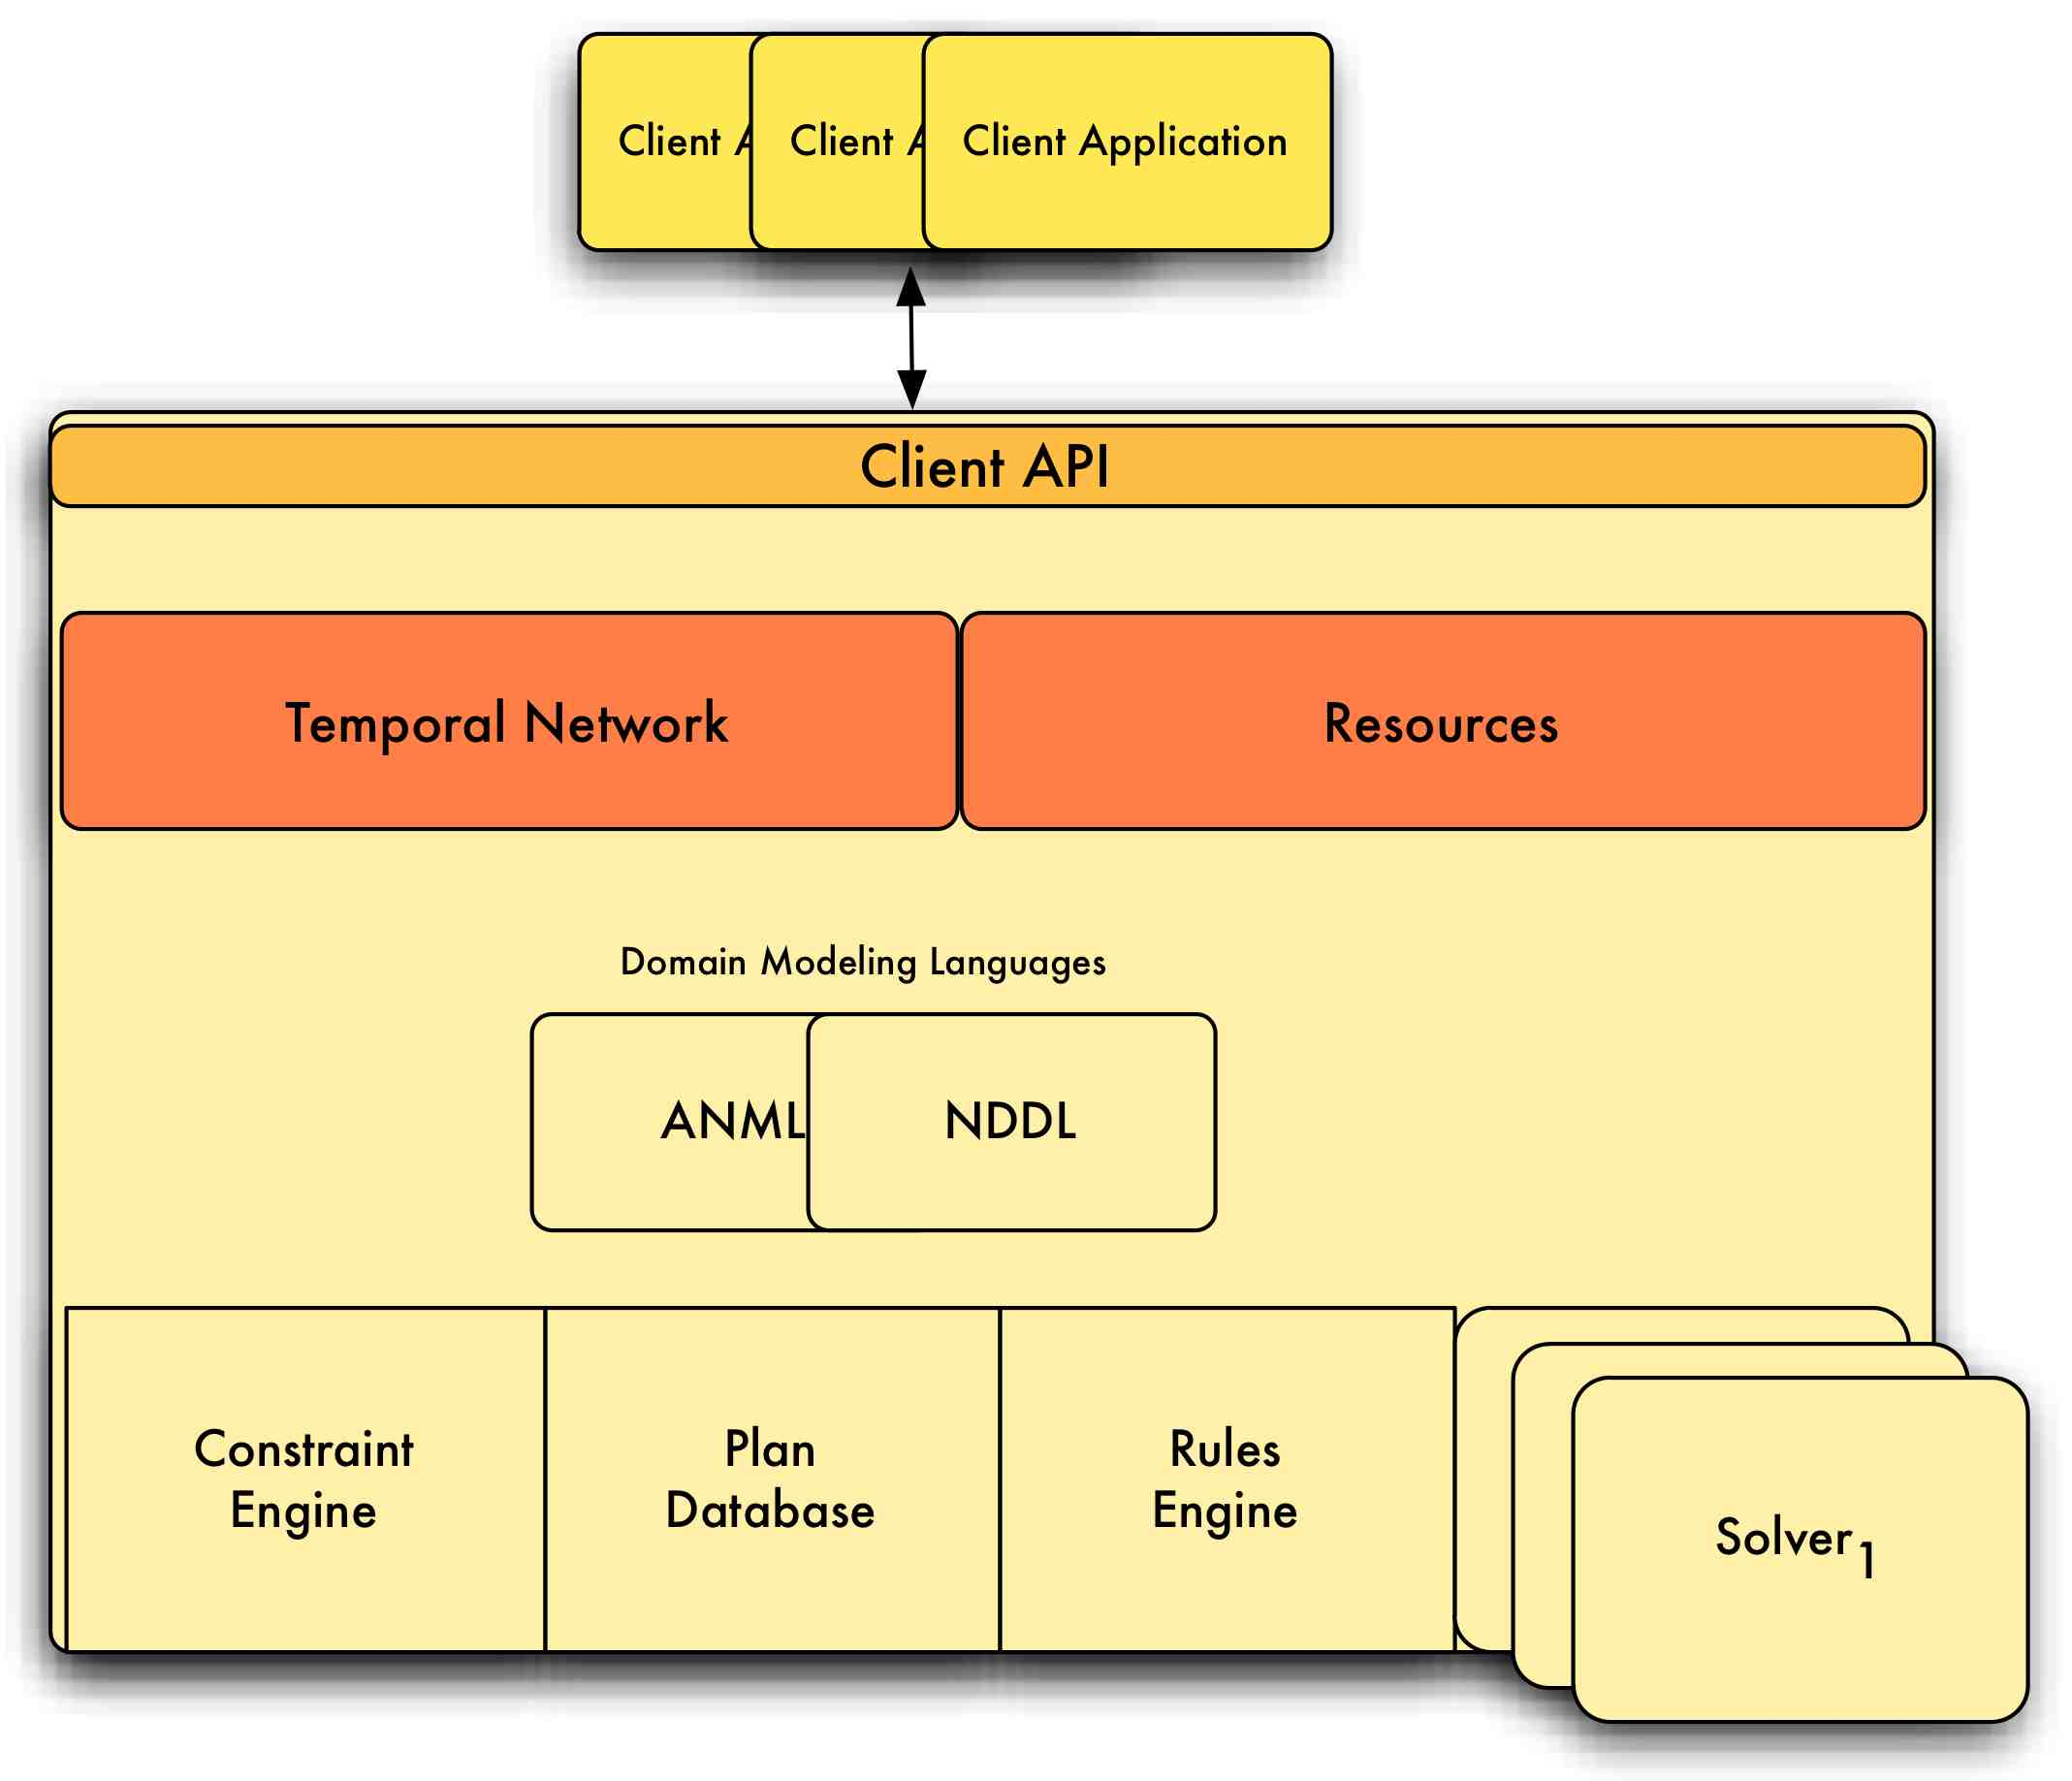
\includegraphics[scale=0.25]{figs/EUROPA-Architecture.jpg}
\caption{\small EUROPA's Architecture}
\label{fig:europa-architecture}
\vskip+0.1cm
\end{figure}


\begin{enumerate}

	\item The Constraint Reasoning Engine (CRE): manages variables, the domains from which they can take values, and constraints that define relationships among variables. It also provides an efficient arc consistency mechanism (TODO: ref to AC-3). The CRE is designed so that specialized reasoning algorithms for specific constraints can be easily and efficiently plugged in.

	\item The Plan Database (PDB): manages object types and objects, which are a mechanism to group variables to more naturally model the real world in much the same way that object oriented programming does. Also manages tokens, which are a mechanism to group variables to represent temporally scoped state. Objects and tokens can be used to model planning domains in a much more natural and extensible way that a pure CSP approach can.

	\item The Rules Engine (RE): manages token relationships in a planning model

	\item The language modules: NDDL, ANML, and other higher level modeling languages can me used to create domain models and problem instances (TODO: point advantages over pure programming API approaches, provide snippets)

	\item API Layer: makes all the services available so that EUROPA can be used to build applications.

\begin{figure}
\centering
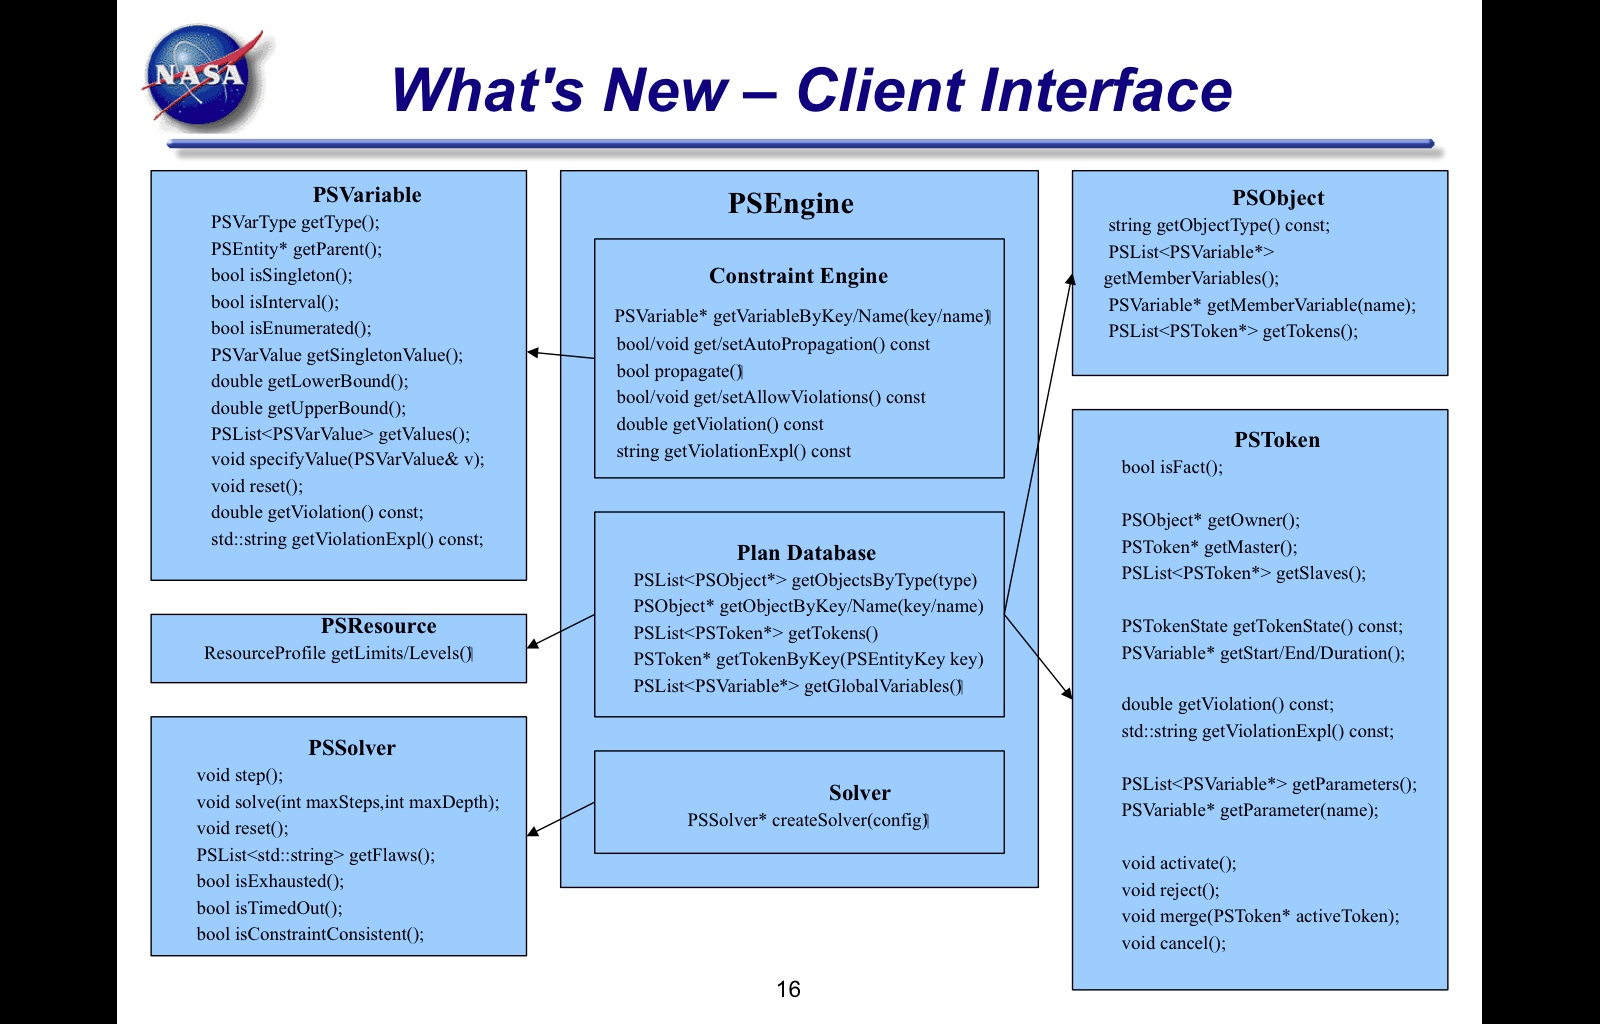
\includegraphics[scale=0.35]{figs/EUROPA-API.jpg}
\caption{\small EUROPA's Client API}
\label{fig:europa-api}
\vskip+0.1cm
\end{figure}


	\item Extension Modules bundled with EUROPA: Temporal Network, Resources, NDDL, ANML.
		\begin{enumerate}
			\item Temporal Network
			\item Resources
			\item NDDL
			\item ANML (TODO:maybe it's better to leave out?)
		\end{enumerate}

\end{enumerate}


\subsection{Modeling}
\label{sec:europa:modeling}

EUROPA can ingest descriptions of models, plans and goals. This means that a single planner can be applied to different systems and problems, simply by providing different models and goals. For such planners the expressiveness of the languages for models, goals and plans is of great importance. EUROPA provides a high level language called NDDL (New Domain Description Language) that allows the user to specify the different components of a problem domain in a concise way. The main characteristics that make NDDL a powerful tool for describing problem domains are:

\begin{enumerate}
	\item It's Object Oriented: NDDL supports classes and inheritance in similar fashion to popular Object-Oriented languages like Java and C++. It also supports polymorphism for some of the planning components. Using object classes and instances is a time-tested approach to naturally describe problem domains (TODO: OO ref?).
	\item It offers declarative constructs to define constraints and causality dependencies between actions and effects.
	\item It offers procedural constructs to populate EUROPA's plan database with specific problem instances expressed in terms of objects, variables, constraints, facts and goals.
\end{enumerate}

To understand how the most important elements of NDDL work, let's take a look at how the Shopping Agent problem described above would be modeled:

\begin{verbatim}

// Locations (Home, SuperMarket, etc.)
class Location {
  string name;
  Location(string _name){
    name = _name;
  }
}

// Products (Milk, Banana, etc.) and
class Product {
  string name;
  Product(string _name) {
    name = _name;
  }
}

// ProductLocations (Banana can be found at SuperMarket, for example)
class ProductLocation {
  Location location;
  Product product;

  ProductLocation(Location _location, Product _product){
    location = _location;
    product = _product;
  }
}

// Use built-in Timeline functionality to enforce that an agent:
// a) Can't be at more than one place at a time.
// b) Can't Go more than one place at a time.
// c) Can't Go somewhere and be At somewhere at the same time.
class AgentLocation extends Timeline{
  predicate At {
    Location loc;
  }

  predicate Going {
    Location from;
    Location to;
  }
}

// In addition to having a location timeline, the agent can buy and own things.  
// Note that the actions and the location predicates can be concurrent 
// so they can't be on the same Timeline
class Agent {
  AgentLocation location;

  Agent() {
    location = new AgentLocation();
  }

  action Buy {
    Product product;
  }
  
  action Go {
    Location from;
    Location to;
  }
  
  predicate Own {
  	Product product;
  }
}


// Define the rules for our actions:
Agent::Go {
  met_by(condition object.location.At origin);
  eq(from, origin.loc);
 
  equals(effect object.location.Going going);
  eq(going.from, from);
  eq(going.to, to);
   
  meets(effect object.location.At destination);
  eq(to, destination.loc);
}

Agent::Buy {
  // A Buy takes 10 time units
  eq(10, duration);

  // initialized to all locations
  ProductLocation possibleStores;

  // limit possibleStores variables to ones that provide what we need to buy
  eq(product, possibleStores.product);

  // We must be At a location during our Buy, and that location must have the
  // product we want available:
  contained_by(condition object.location.At currLocation);
  eq(currLocation.loc, possibleStores.location);
  
  starts(effect Own purchase);
  eq(purchase.product,product);
}

\end{verbatim}

TODO: explain variable, object, predicate and action types, including constraints that can be part of them

In this model we can see:

\begin{enumerate}
	\item Variable Types: This model uses integer (activity duration, start and end times, etc) and string (Location and Product names, etc)
	\item Object Types:
	\item Predicate Types:
	\item Action Types:
\end{enumerate}


Now let's look at how a specific problem instance would be specified in NDDL:

\begin{verbatim}

// Allocate instances
Location Home = new Location("Home");
Location SuperMarket = new Location("SuperMarket");
Location HardwareStore = new Location("HardwareStore");

Product Banana = new Product("Banana");
Product Milk = new Product("Milk");
Product Drill = new Product("Drill");

ProductLocation bananaLocation = new ProductLocation(SuperMarket, Banana);
ProductLocation milkLocation = new ProductLocation(SuperMarket, Milk);
ProductLocation drillLocation = new ProductLocation(HardwareStore, Drill);

Agent agent = new Agent();

// Indicate that the database is closed - no new objects can be created
// this allows EUROPA to perform more efficient inference
close();

// We start the day at Home:
fact(agent.location.At atHomeForBreakfast);
atHomeForBreakfast.loc.specify(Home);

// Goals for all of the agent's needs, buy if needed
goal(agent.Own gotMilk);
gotMilk.product.specify(Milk);
goal(agent.Own gotBanana);
gotBanana.product.specify(Banana);
goal(agent.Own gotDrill);
gotDrill.product.specify(Drill);

// Make sure agent is home for dinner
goal(agent.location.At atHomeForDinner);
atHomeForDinner.loc.specify(Home);

// Agent has all day to satisfy goals:
gotMilk after atHomeForBreakfast;
gotMilk before atHomeForDinner;

gotBanana after atHomeForBreakfast;
gotBanana before atHomeForDinner;

gotDrill after atHomeForBreakfast;
gotDrill before atHomeForDinner;

// Force things to happen within our planning horizon:
int horizonStart = 0;
int horizonEnd = 100;
leq(horizonStart, atHomeForBreakfast.start);
leq(atHomeForDinner.end, horizonEnd);

\end{verbatim}

TODO:  explain variable, object, predicate and constraint instances.
explain goals and facts.

\begin{enumerate}
	\item Variable Instances:
	\item Object Instances:
	\item Facts:
	\item Goals:
	\item Constraint Instances:
\end{enumerate}


\subsection{Inference}
\label{sec:europa:inference}

TODO: explain how inference is used to detect perform bounds propagation, domain reduction and to detect constraint violations.
- talk about AC3 implementation and extension mechanisms
- talk about europa's constraint library


The Temporal Network:
The notion of time is central to temporal planning. EUROPA uses variables to explicitly represent timepoints for plan activities and states. Constraints among timepoints provide a natural way to express domain axioms. For example, in order to state that activity A must occur before activity B we can say that the end timepoint of A is <= the start timepoint of B. 

\begin{figure}
\centering
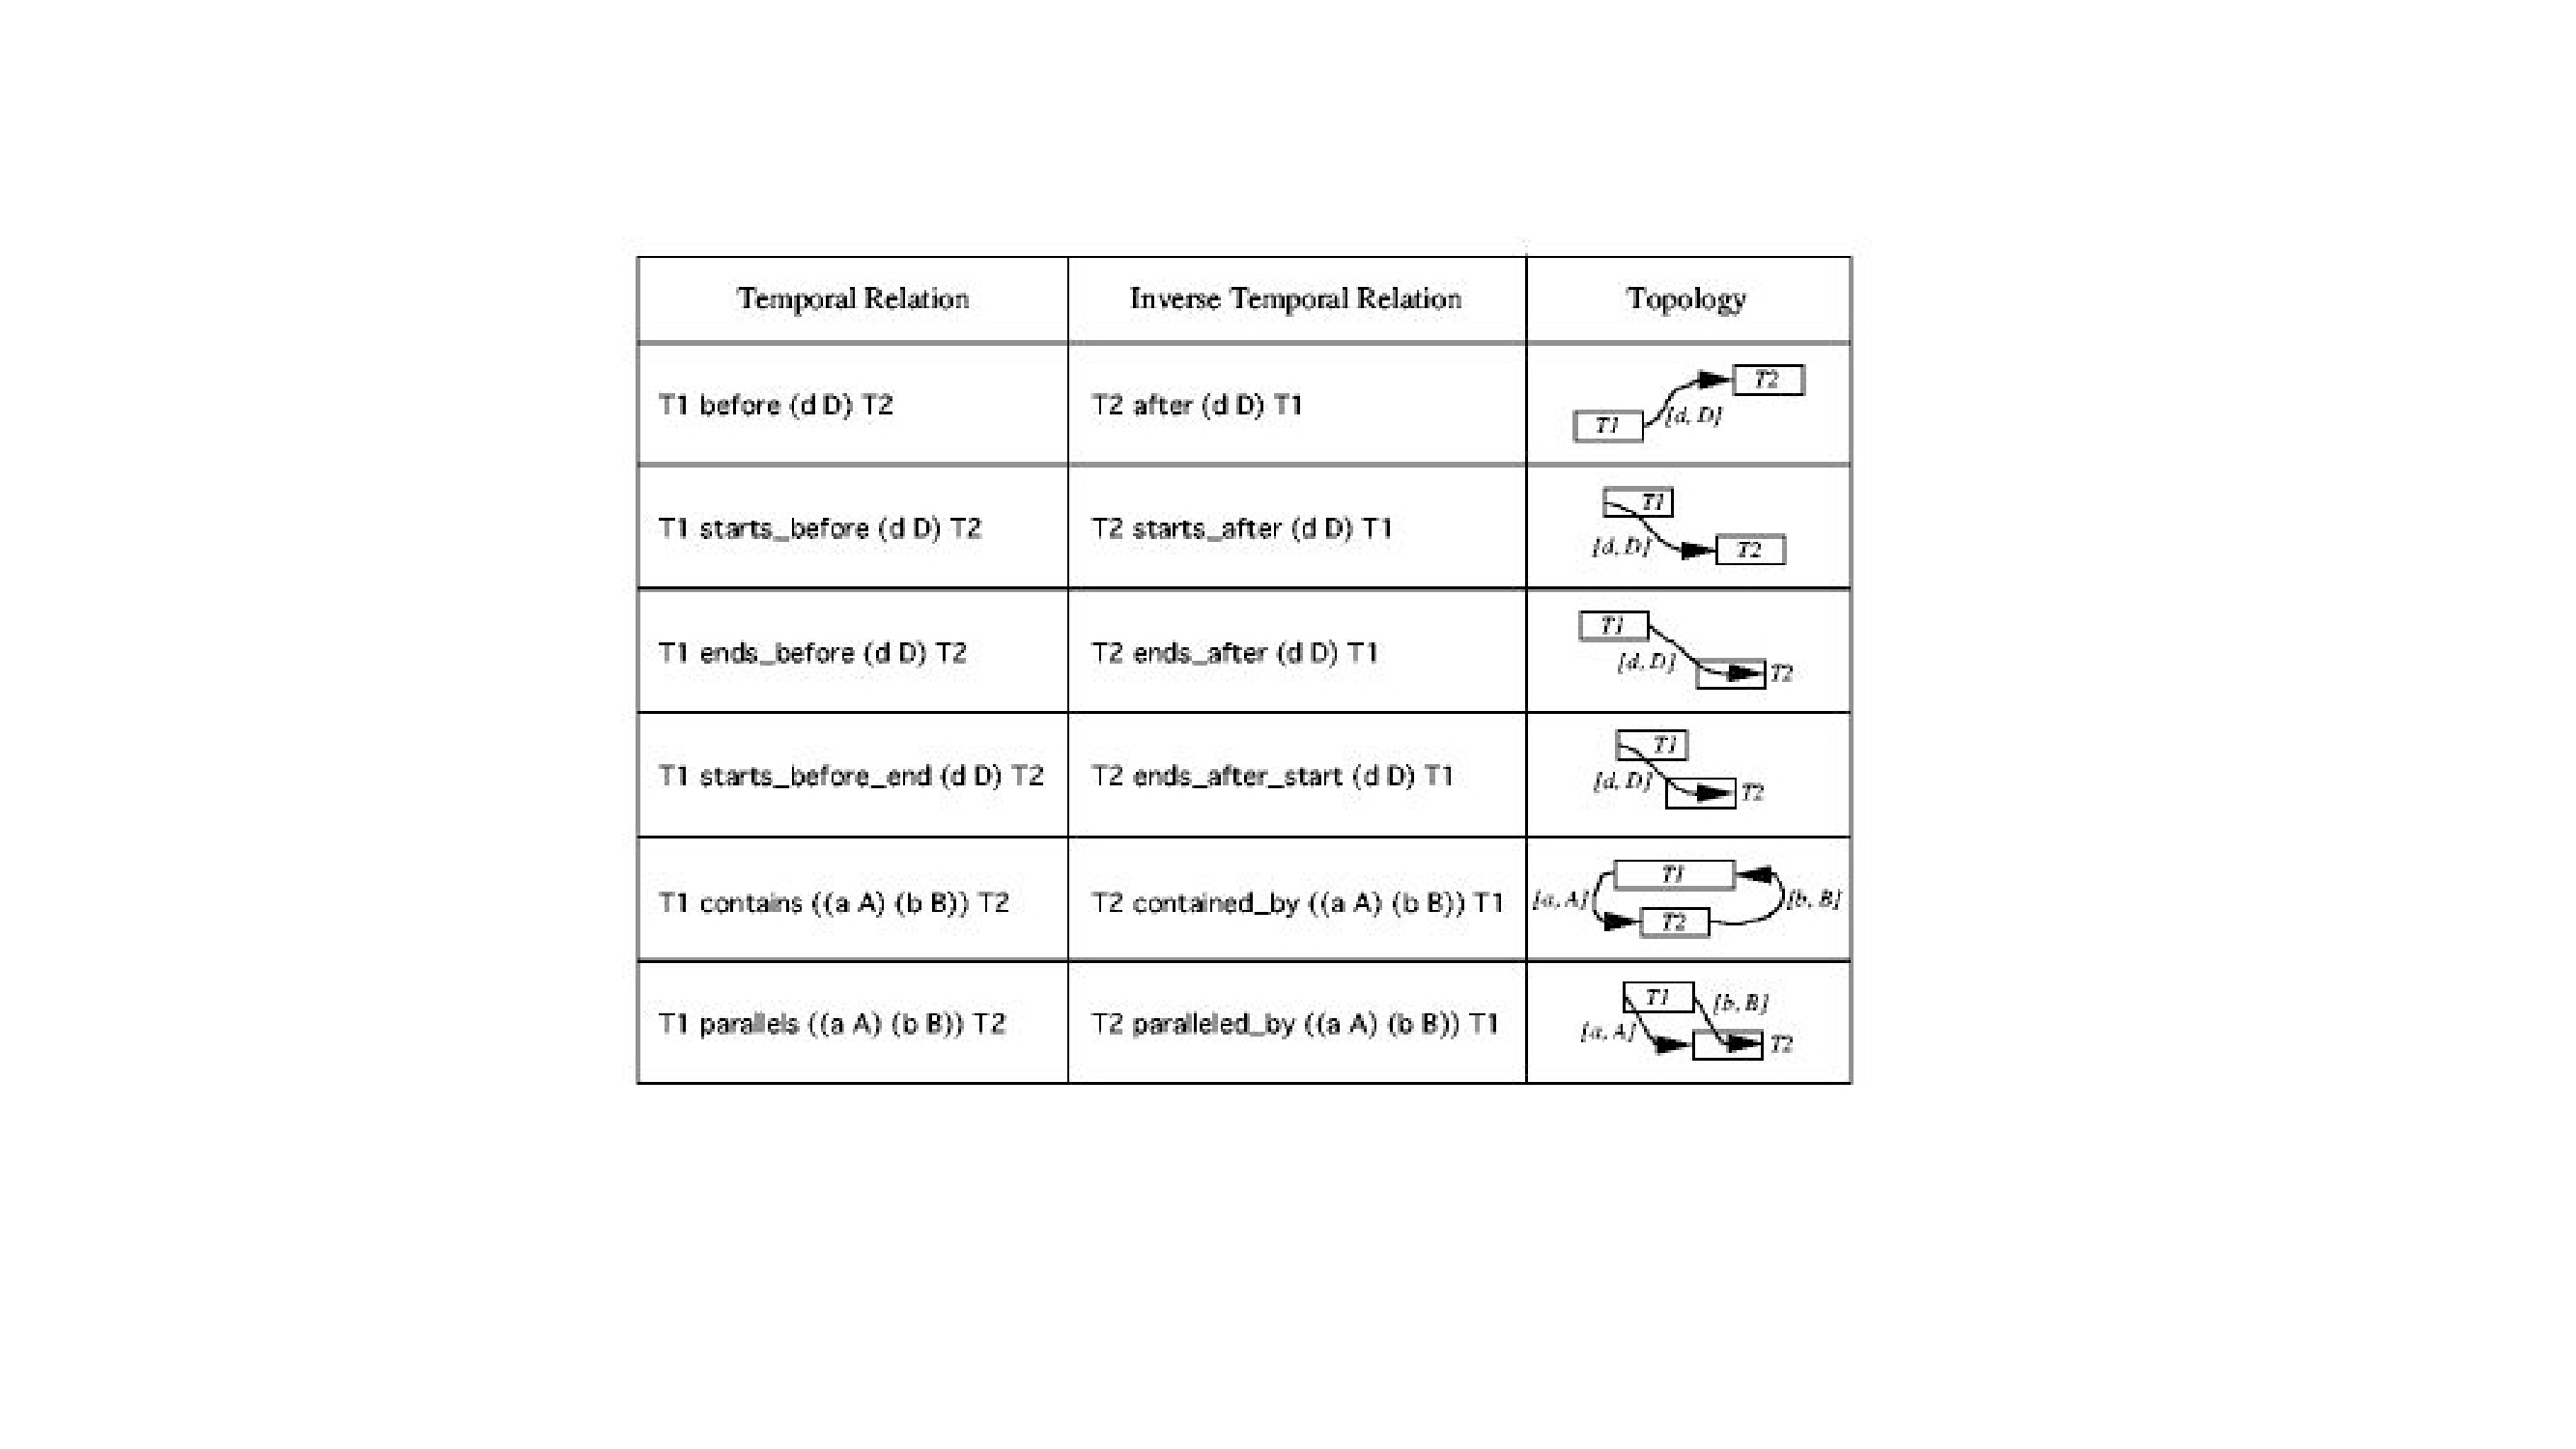
\includegraphics[scale=0.3]{figs/Allen-algebra.pdf}
\caption{\small Temporal relations defined within the planner are
  based on \texttt{Allen Algebra} relations shown above.}
\label{fig:allen-algebra}
\vskip-0.3cm
\end{figure}

Dechter et al. (Dechter 1991) proposed that constraints among timepoints can be grouped together to form a Simple Temporal Network (STN). Such a network can be transformed into a Distance Graph (DG) where the outward arc from a node represents the maximum distance from the source node to the target node. The diagram below illustrates a simple STN with just 2 variables and a single constraint. It also shows the resulting DG. 

TODO: add figure

Dechter et al. (Dechter 1991) also showed that shortest path algorithms could be used to propagate values in the network and discover a negative cycle. A negative cycle is a path from a node to itself that has a path length less than 0. If such a cycle exists, the network is inconsistent. It was further shown that a single-source shortest path algorithm was sufficient to detect a negative cycle and provide sufficient propagation to yield a backtrack-free search. Thus we have an efficient and complete algorithm for propagating an STN. These results build on the already established notion of a CSP and are naturally incorporated into the general representation and propagation scheme used in EUROPA. 

Resources:

    Reservoir resources can have both 'consume' and 'produce' tokens. Note that these tokens do NOT have the usual start/end/duration token variables, since occur at a single instant in time. Instead, they have a single variable, 'time' used to represent that instant.
    Reusable resources have 'uses' tokens that use a quantity for the duration of the token. These tokens do have the usual start/end/duration variables.
    Unary resources are reusable resources with unit quantity and have 'use' tokens (again, with the usual start/end/duration variables). 
    
    TODO: talk about resource envelope computation by using MaxFlow formulation.


\subsection{Search}
\label{sec:europa:search}

Now we have all the elements in place so that an automated problem solver can be created. Let's recap what those elements are:

\begin{enumerate}

\item A domain model that describes the variable, object, predicate and action types that are relevant for the problem.
\item A problem instance (also called initial state) that consists of:
	\item Variable and Object instances that exist for the entire planning horizon.
	\item Temporally scoped predicate and action instances.
	\item Temporally scoped goals.

\end{enumerate}
	
All this information is kept in EUROPA's  Plan Database so that inference and search mechanisms can be used to look for a problem solution.

Given that temporal intervals may extend indefinitely in both positive and negative directions, for problems with a temporal dimension it is also common to specify a Planning Horizon when invoking a solver. The Planning Horizon is the temporal interval that a problem solver has to worry about, any decisions that fall completely outside of the Planning Horizon can be ignored. This is very useful for recurrent activities, consider for instance a model where a medical checkup has to occur every 3 months, the user can model a recurring activity and then use the Planning Horizon to ensure that a finite number of medical checkup activities are generated as part of a plan. This is also useful to ignore activities that may happen too far in the future or in the past to be relevant for a particular plan, this way the user can ensure that the solver is making as few commitments as necessary.

EUROPA provides a built-in solver that performs Plan Space Planning (TODO: ref), in this approach, the initial state is considered a partial plan that needs to be refined toward a solution plan that achieves the goals. The operations to refine the partial plan PP at any time are:
\begin{enumerate}
	\item Find the flaws of PP, that is the conditions that prevent it from being a solution plan (flaw types are explained below).
	\item Select one such flaw
	\item Select a resolver for the flaw
	\item Refine PP by applying the resolver
	\item If an inconsistency is found, try another resolver.
	\item If all possible resolvers for a particular flaw fail, return failure, otherwise continue until resolving all the flaws.
\end{enumerate}
	
This Plan Space Planning algorithm is translated into EUROPA's representation as follows:

The initial partial plan is the state of EUROPA's Plan Database after the initial state has been instantiated, this results in a set of variable, object and token instances. Inference then takes place to detect flaws in the partial plan, there are 3 kinds of flaws that can be detected:

\begin{enumerate}
	\item Unbound Variable: a variable in the partial plan whose domain is not a singleton. Unbound Variables are resolved by specification of a value from the domain of the variable.

	\item Open Condition: an open condition is an inactive token. Inactive tokens can be generated by explicitly posted goals, or when a token is activated, rules may fire that create inactive slave tokens (TODO: point to more detailed decription above in Rules Engine section).  Open Conditions can be resolved in three ways: 
\begin{enumerate}
		\item Merging: A free activity is merged with a matching activity already in the plan. An activity a is said to match an activity a? if a and a? unify and the temporal constraints involving a are satis�ed by a?. Thus,  a and a? can be considered the same activity and we do not need to introduce a in the plan. Consequently, the compatibilities associated with a are not �red, because they have been already triggered when a? was introduced in the plan. 
		\item Activation: We introduce a new activity a in the current plan associating it with the proper timeline, but without choosing a speci�c time slot for it.The compatibilities associated with a are applied and the subgoal activities resulting from those compatibilities are introduced as free activities. This results in both an ordering �aw, corresponding to the just activated activity, and a number of open condition �aws, corresponding to the new subgoal activities. 
		\item Rejection: Some goals may be optional, if that is the case for a particular order condition, its corresponding flaw can be resolved by discarding the inactive token.
\end{enumerate}

	\item Threat: once a token has been placed in the partial plan it may impact other tokens indirectly through possible overlapping requirements on objects. Recall for example that a token may belong to objects (e.g. Timelines) which require a total order over their tokens. If any 2 tokens could possibly overlap (though not necessarily), then they pose a threat to each other in terms of achieving an extension of the current partial plan which is complete and consistent. Similarly, threats may arise where tokens share a common resource and their current state might yield extensions of the current partial plan which are inconsistent. Threats are resolved by imposing ordering constraints among tokens. 

\end{enumerate}

Open Conditions and Threats allow flaw detection and resolution at a higher-level of abstraction (i.e. in terms of objects and tokens) than that of simply binding variables as is common in Constraint Satisfaction Problems. This is advantageous when one applies heuristics for ordering choices since it provides a richer context in which to make decisions. Furthermore, it aids in reducing the amount of work done by a solver so that only the necessary refinements are made, otherwise leaving the partial plan with maximum flexibility. For example, one can omit unbound variables which are time-points of tokens since threats will force a solver to impose restrictions on these variables based on the semantics of the objects to which their tokens apply. Thus the planning process may yield partially-ordered plans for which all possible extensions are provably valid. 

The Plan Space Planning algorithm described above can be implemented in many different ways depending on the approach chosen for flaw and resolver selection and for backtracking. EUROPA's built-in solver implements a chronological backtracking algorithm that is summarized in the figure below.

\begin{verbatim}

01.  bool solve(PartialPlan plan)
02.   {
03.      if (isInconsistent(plan))  return false;
04.
05.      Flaw flaw = chooseFlaw(plan);
06.      if (flaw == NULL) return true;
07.
08.      DecisionPoint decision = makeDecisionPoint(flaw, plan);
09.
10.      while(decision.hasNext()) {
11.          PartialPlan pp = decision.executeNext();
12.
13.          if (solve(pp)) return true;
14.          else d.undo();
25.      }
16.
17.      return false;
18.  }

\end{verbatim}

The algorithm takes as input a partial plan p and returns true if a complete and consistent refinement of p could be found (or if p is initially complete and consistent), and false otherwise. 

\begin{enumerate}
	\item Line 3: Propagate the constraints to test for inconsistency. If found to be inconsistent, then we can return false since this is a dead-end i.e. no refinements to p can yield a consistent plan.
	\item Line 5: Choose a flaw from the set of available flaws.
	\item Line 6: If there are no flaws, then p is complete and we can terminate with success.
	\item Line 8: Otherwise we formulate a decision point which is a branch in the search space. Each choice is a particular refinement operation and the DecisionPoint collects all possible refinement operations for the given flaw.
	\item Line 10: We keep trying until the chosen flaw is resolved, or until we run out of resolvers to try.
	\item Line 11: A new partial plan is obtained by application of a refinement operator. Note that the ordering over refinement operators to select is a non-deterministic step.
	\item Line 13: Recursive call to solve the new planning problem. If successful, then we are done.
	\item Line 14: Otherwise, retract the last refinement operation and move on to try the next one.
	\item Line 17:  If we arrive here, then we have exhausted all options to resolve the flaw, including the case where no options were available initially. Thus the problem cannot be solved.
\end{enumerate}

This algorithm provides for a sound and complete search, assuming that no flaws or available refinement operators are pruned unnecessarily. Dead-ends in the search are discovered through constraint propagation. Constraint propagation is a vehicle for evaluating the consistency of a partial plan and also for filtering infeasible values from consideration prior to commitment, allowing in some cases a strong look-ahead capability which is essential for tractable search. Consistency testing is initiated by the isConsistent procedure. The algorithm permits a heuristically controlled search by applying orderings for chooseFlaw and makeDecisionPoint. It results in a chronologically-backtracking, search. 

TODO: expand a little more on how heuristics can be implemented by applying ordering/filtering for chooseFlaw and makeDecisionPoint
examples:
- deal with earliest flaws first
- deal with planning (open condition flaws) before scheduling (threats) ones

It should be emphasized that while this algorithm is commonly employed, it is only one of many that could be implemented. TODO: give examples of local search solvers for scheduling and CSP?

N-Queens solver:
\begin{verbatim}
    public void solve(int maxIter)
    {
    	init();
    	
    	for (int i=0;psengine_.getViolation() > 0 && i < maxIter;i++) {
    	    PSVariable queenToMove = getQueenWithMaxViolation();
    		int curPos = queenToMove.getSingletonValue().asInt();
    	    
    	    boolean moved = false;
            SortedSet<Move> moves = getMoves(queenToMove,curPos);             
            for (Move m : moves) {
            	moved = makeMove(queenToMove,curPos,m,false);
            	if (moved)
            	    break;
            }
            
            if (!moved) 
            	makeMove(queenToMove,curPos,moves.first(),true);
            
            checkSolution(); // See if we have a new best solution            
            notifyIterationCompleted(curIteration_++);
            
            if (curIteration_-bestIter_ > 50) 
            	restart();
    	}
    }
\end{verbatim}

RCPSP solver:
\begin{verbatim}
    public void solve(PSEngine psengine,
    		          long timeout, // in msecs
    		          int bound)
    {
       init(psengine,timeout,bound);
       
       for (int i=0; true ; i++) {
          flatten();
          updateSolution(i);
          updateCriticalPrecedences();
          
          if ((nbStable_ > maxStable_) || (bestMakespan_ <= makespanBound_))
             break;
          
          if (timer_.getElapsed() > timeout) {
              timedOut_ = true;
              break;
          }
          
          relax();
          curIteration_++;
       }       

       restoreBestSolution();
    }

\end{verbatim}


TODO: 
- explain how other solvers can be built, maybe use NQueens or RCPSP example to illustrate. Or maybe build a little specialized solver for shopping or rover examples.


%%% Local Variables: 
%%% mode: latex
%%% TeX-master: "setobook"
%%% End: 


 